\subsection{Généralité}	
Ce stage réalisé dans le cadre de ma 2$^{eme}$ année de Master Informatique fut l'occasion de poursuivre mon travail dans le domaine de la santé débuté durant mon TER. Succintement, ce travail consistait en l'expérimentation de l'utilisation de technologies informatiques pour l'évaluation des capacités motrices de patients hémiplégiques. Ce projet de TER a été réalisé avec William DYCE, par ailleurs stagiaire avec moi chez NaturalPad. Nous avons conçu un prototype d'application permettant, grâce à la Kinect, de juger de la réussite ou non de plusieurs des exercices d'évaluation du test de %\gls{fuglmeyer} 
par un patient en réhabilitation suite à un AVC. \paragraph{}
Fort de cette expérience et vivement motivé par le fait de travailler dans un contexte médical, ce stage constituait une excellente opportunité d'orienter ma formation vers le développement d'applications et de jeux pour la santé.\\
L'objectif de ce stage était de proposer un moyen ou des outils pour adapter la difficulté de jeux sérieux pour la santé dans le domaine de la rééducation motrice. Nous verrons que différentes approches sont possibles et quelle fut démarche lors de ce stage. Par ailleurs, ce fut pour moi l'occasion de m'insérer dans le projet de grande envergure, Hammer \& Planks, et de participer à mes deux premières GameJam, comme je le détaillerai en annexe.

\subsection{L'entreprise}
	\subsubsection{Naturalpad}
NaturalPad est une jeune startup innovante basée dans la région de Montpellier. Elle est spécialisée dans les technologies appliquées à la santé et développe notamment des jeux vidéos à but thérapeutique pour la rééducation fonctionnelle. Ces jeux utilisent des technologies de capture du mouvement grand public comme le Kinect de Microsoft ou la Wii Board de Nintendo. L’idée de Naturalpad est née lors du projet MoJOS (Moteur de Jeux Orienté Santé), pionnier en matière de projet de recherche serious game, sur lequel plusieurs membres de l’équipe ont travaillé. En effet, prenant conscience du marché porteur des serious games et plus largement de celui de la santé, Antoine Seilles et les 4 autres fondateurs ont créé le projet NaturalPad en se démarquant des concurrents par une volonté de faire avant tout du jeu, bien qu’il soit sérieux, et d’y apporter une dimension sociale. L’idée au delà du développement de jeux est de proposer un système sous forme de plateforme intégrant plusieurs jeux thérapeutiques. Ceux-ci permettant au patient de suivre sa thérapie à domicile tout en jouant avec ses proches (ils sont considérés dans la conception du gameplay) et donnant la possibilité au thérapeute de suivre la progression du patient. NaturalPad a par ailleurs signé un partenariat avec le Centre Hospitalier Alès Cévennes (CHAC) dans le but de développer des services web innovants pour les équipes de pédiatrie, néonatalogie et gériatrie du CHAC. Le CHAC peut être considéré comme le site pilote des produits NaturalPad. Un partenariat de recherche a été mis en place avec deux laboratoires de recherche de Montpellier que sont le LIRMM (Laboratoire d’Informatique, de Robotique et de Microélectronique de Montpellier) et le M2H (Movemement 2 Health : Laboratoire en Sciences du Mouvement) dans le cadre des activités de NaturalPad.

	\subsubsection{L'équipe}
	\begin{figure}[!h]
		\centering
		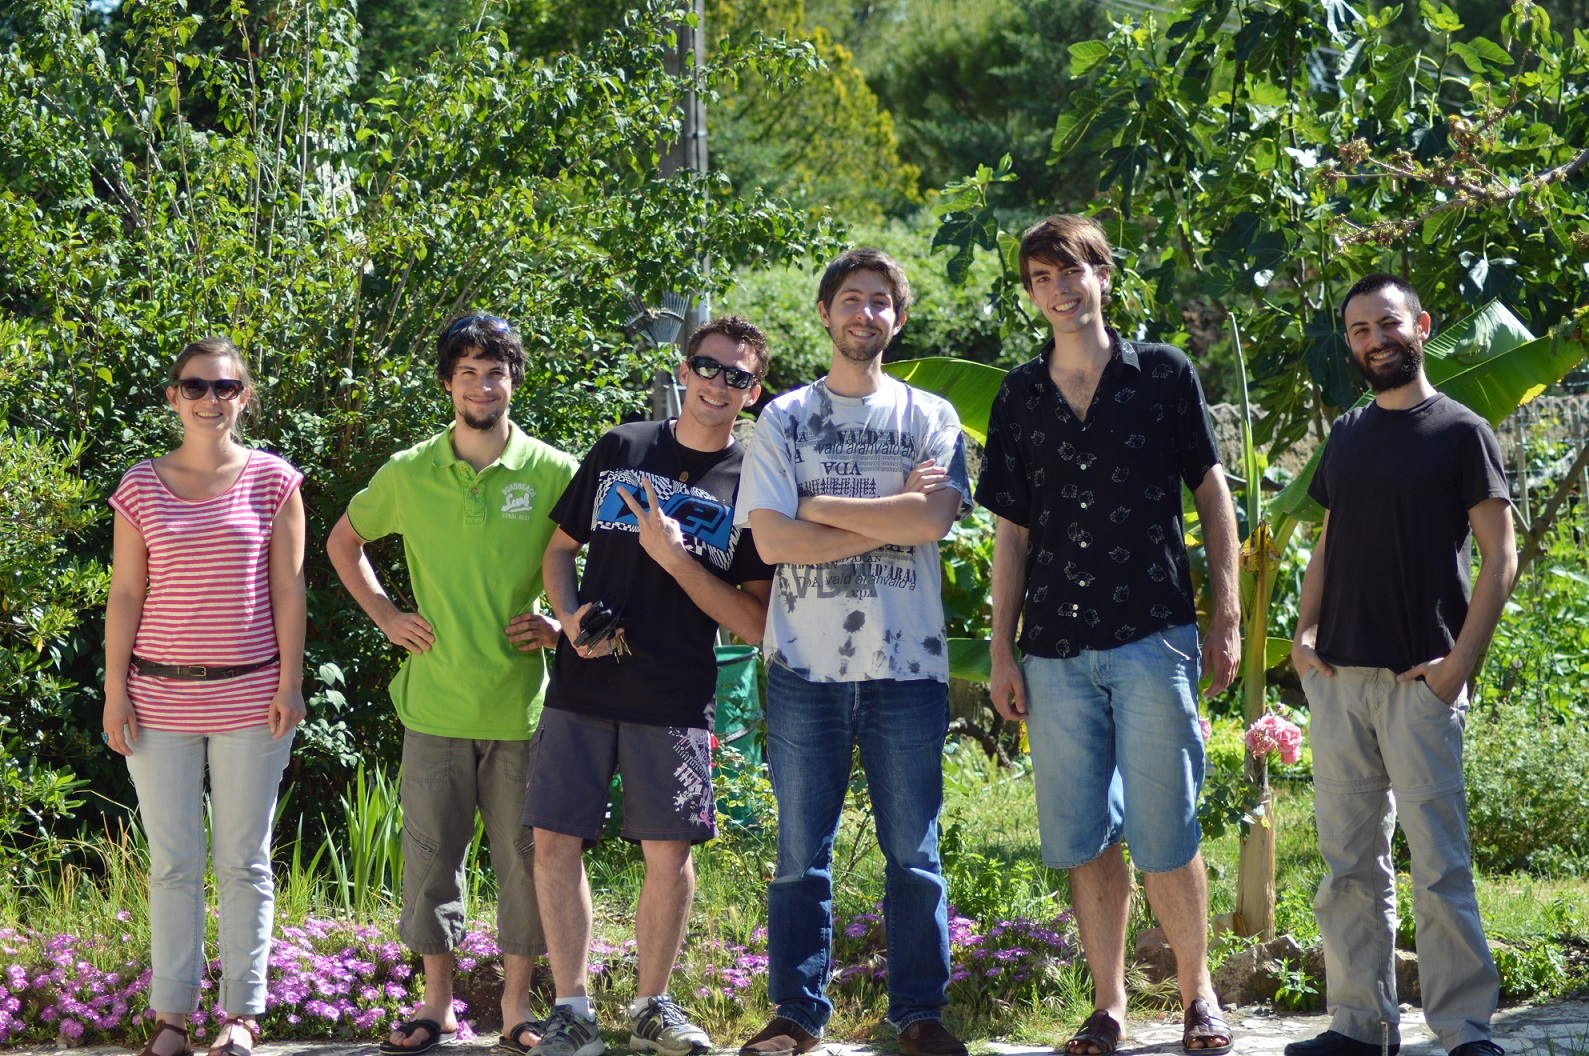
\includegraphics[width=420px]{images/naturalpad_groupe.jpg}
		\caption{L'équipe de NaturalPad à Prades le Lez}
		\label{naturalpad_groupe}
	\end{figure}
	
		\subsubsection*{Antoine SEILLES - Fondateur}
\begin{minipage}[t!]{0.2\linewidth}
\centering

\includegraphics[width=0.8\textwidth]{images/tetocarre/antoine}
\end{minipage}
\begin{minipage}[t!]{0.79\linewidth}
Docteur en informatique, il a soutenu sa thèse en 2012, portant sur les usages du Web 3.0 (ou web socio-sémantique) dans le contexte de la démocratie électronique. 
		\begin{quotation} \emph{Au sein de NaturalPad} \end{quotation}
Antoine est le PDG de NaturalPad et gère la société au quotidien.
\end{minipage}

		\subsubsection*{Sébastien ANDARY - Fondateur}
\begin{minipage}[t!]{0.2\linewidth}
\centering

\includegraphics[width=0.8\textwidth]{images/tetocarre/seb}
\end{minipage}
\begin{minipage}[t!]{0.79\linewidth}
Il a reçu le diplôme de Master d’Informatique à l’Université de Montpellier et termine actuellement un Doctorat de Robotique au LIRMM. Sa thèse porte sur la commande des systèmes mécaniques sous-actionnés dans le cadre de la robotique humanoïde. 
		\begin{quotation} \emph{Au sein de NaturalPad} \end{quotation}
Sébastien travaille au développement de technologies et outils innovants pour la captation de mouvements.
\end{minipage}

		\subsubsection*{Inès DI LORETO - Fondatrice}
\begin{minipage}[t!]{0.2\linewidth}
\centering

\includegraphics[width=0.8\textwidth]{images/tetocarre/ines}
\end{minipage}
\begin{minipage}[t!]{0.79\linewidth}
Elle est diplômée en philosophie et a obtenu un doctorat en informatique à l’Università degli Studi di Milano (Italie). Fin 2009, elle rejoint en postdoc le projet \href{http://www.mojos.fr}{MoJOS}. Dans ce projet de recherche sur les jeux thérapeutiques elle a mené des activités scientifiques pour relever les défis de l’acceptation des patients et des thérapeutes du jeu comme moyen de rééducation. 
		\begin{quotation} \emph{Au sein de NaturalPad} \end{quotation}
Inès travaille sur la transformation des objectifs thérapeutiques en objectifs de jeu en collaboration directe avec les professionnels de la santé.
\end{minipage}

		\subsubsection*{Tristan LE GRANCHE - Fondateur}
\begin{minipage}[t!]{0.2\linewidth}
\centering

\includegraphics[width=0.8\textwidth]{images/tetocarre/tristan}
\end{minipage}
\begin{minipage}[t!]{0.79\linewidth}
Travaillant dans le monde du cinéma d’animation depuis plus de 4 ans, il a travaillé sur plus d’une dizaine de projets de séries télévisées, et de longs et courts métrages. Aujourd’hui il s’est spécialisé dans les Effets Spéciaux Numériques et travaille à l’international en tant que Directeur Technique.
		\begin{quotation} \emph{Au sein de NaturalPad} \end{quotation}
Tristan occupe le poste de Directeur Artistique.
\end{minipage}
	
		\subsubsection*{Benoit LANGE - Fondateur}
\begin{minipage}[t!]{0.2\linewidth}
\centering

\includegraphics[width=0.8\textwidth]{images/tetocarre/ben}
\end{minipage}
\begin{minipage}[t!]{0.79\linewidth}
Il est diplômé d’un master informatique spécialisé en Web et Intelligence Artificielle. Il a ensuite obtenu son diplôme de docteur en informatique à l’université Montpellier 2 en Novembre 2012. Ce doctorat avait pour sujet de réaliser une méthode de visualisation de données afin de permettre l’optimisation énergétique pour le bâtiment. 
		\begin{quotation} \emph{Au sein de NaturalPad} \end{quotation}
Benoit propose, étudie et met en oeuvre des prototypes d’interactions adaptés à des thérapies.
\end{minipage}

		\subsubsection*{Anthony BARREAU - Employé}
\begin{minipage}[t!]{0.2\linewidth}
\centering

\includegraphics[width=0.8\textwidth]{images/tetocarre/anthony}
\end{minipage}
\begin{minipage}[t!]{0.79\linewidth}
Il est diplômé d’une licence professionnelle en informatique spécialité web et gestion. Il a ensuite débuté son expérience professionnelle au sein de l’équipe SMILE du LIRMM. Il a rejoint l’équipe pour participer au développement du projet \href{http://www.mojos.fr}{MoJOS}. Dans ce projet de recherche sur les jeux thérapeutiques, il a participé au développement de prototypes de jeux et d’agents intelligents servant à adapter la difficulté. 
		\begin{quotation} \emph{Au sein de NaturalPad} \end{quotation}
Anthony participe au prototypage et au développement des outils innovants de l’entreprise.
\end{minipage}

		\subsubsection*{Marion FLORIS - Employée}
\begin{minipage}[t!]{0.2\linewidth}
\centering

\includegraphics[width=0.8\textwidth]{images/tetocarre/marion}
\end{minipage}
\begin{minipage}[t!]{0.79\linewidth}
Titulaire d’un D.U.T. Information-Communication et d’une Licence Professionnelle Management des Ressources Numériques, Marion est issue d ’une formation littéraire. Après avoir été libraire spécialisée en bande dessinée pendant deux ans, elle a développé son expertise en Community Management par une formation de 6 mois chez Objectif3D.
		\begin{quotation} \emph{Au sein de NaturalPad} \end{quotation}
Marion est Community Manager et est chargée de la communication.
\end{minipage}

		\subsubsection*{William DYCE - Stagiaire}
\begin{minipage}[t!]{0.2\linewidth}
\centering

\includegraphics[width=0.8\textwidth]{images/tetocarre/william}
\end{minipage}
\begin{minipage}[t!]{0.79\linewidth}
William effectue son stage de Master 2 IMAGINA en même temps que moi chez NaturalPad. L'objectif de son stage était de permettre une reconnaissance des joueurs et de leurs mouvements plus fine avec la Kinect. L'utilisation du Kinect dans un contexte thérapeutique exige en effet une reconnaissance avec des contraintes plus poussées que pour une utilisation purement ludique. Grâce à cela, il sera possible d’imaginer de nouveaux gameplay de jeux basés sur le mouvement.
\end{minipage}

		\subsubsection*{Andy CAMICCI - Stagiaire}
\begin{minipage}[t!]{0.2\linewidth}
\centering

\includegraphics[width=0.8\textwidth]{images/tetocarre/andy}
\end{minipage}
\begin{minipage}[t!]{0.79\linewidth}
Étudiant en licence professionnelle Activité et Techniques de Communication à Arles, Andy a effectué un stage de trois mois de Avril à Juin durant lesquels il a participé au développement de l'interface web thérapeutique et aux modules de visualisation des données de jeux. Nous avons travaillé conjointement afin de fournir un outil ergonomique et efficace pour la paramétrisation des parties des jeux thérapeutiques présents sur la plateforme.
\end{minipage}
		
		\subsubsection*{Kevin BRADSHAW- Stagiaire}
\begin{minipage}[t!]{0.2\linewidth}
\centering

\includegraphics[width=0.8\textwidth]{images/tetocarre/kevin}
\end{minipage}
\begin{minipage}[t!]{0.79\linewidth}
Actuellement en stage, Kevin est en licence Informatique et souhaite devenir developpeur de jeux vidéo. Durant son stage, il concoit et développe son propre jeu de manière indépendante : Zether. Pour cela, il crée les assets graphiques, le son et les diverses fonctionnalités du jeu. \\
Ce jeu a pour dessein de venir se greffer sur la plateforme web de NaturalPad. Kevin a en effet imaginé un gameplay jouable à la fois avec souris+clavier et par les mouvements du corps avec une caméra Kinect. Utilisant une approche différente de la mienne, l'objectif thérapeutique n'est pas clairement défini bien que pris en compte. La plateforme de NaturalPad veut aussi pouvoir accueilir des jeux qui ne sont initialement pas développés dans une optique de rééducation mais dont une telle utilisation est possible.
\end{minipage}
		
		\subsubsection*{Célia GIRONNET - Stagiaire}
\begin{minipage}[t!]{0.2\linewidth}
\centering

\includegraphics[width=0.8\textwidth]{images/tetocarre/celia}
\end{minipage}
\begin{minipage}[t!]{0.79\linewidth}
Stagiaire infographiste, cette étudiante de SupInfoGame contribue à enrichir le monde de Hammer \& Planks en réalisant les modèles 2D et 3D des personnages, monstres et autres décors de cet univers de pirates !
\end{minipage}

	\subsection{Hammer \& Planks}
Hammer \& Planks est le premier jeu sérieux pour la santé de NaturalPad. Il a été conçu en collaboration avec une ergothérapeute, Anaïs Ivorra, dans le but de permettre aux personnes hémiplégiques de retrouver leur faculté d’équilibre. Il a été présenté à diverses occasions lors de salons, qu’ils soient grand public comme le MIG ou spécialisés (\href{http://www.ted.com/tedx/events/5188}{TEDx Montpellier} / \href{http://www.e-virtuoses.net/}{e-virtuoses}). Il a par ailleurs été primé aux e-virtuoses 2013 de Valenciennes dans la catégorie "Serious Game Healthcare" et est largement cité dans un article composé d'une vidéo sur les Serious Game thérapeutiques sur le \href{http://videos.doctissimo.fr/sante/recherche/serious-game-therapeutique.html}{site de doctissimo}.
		
\begin{figure}[htbp]
	\begin{minipage}[c]{.45\linewidth}
		\begin{center}
			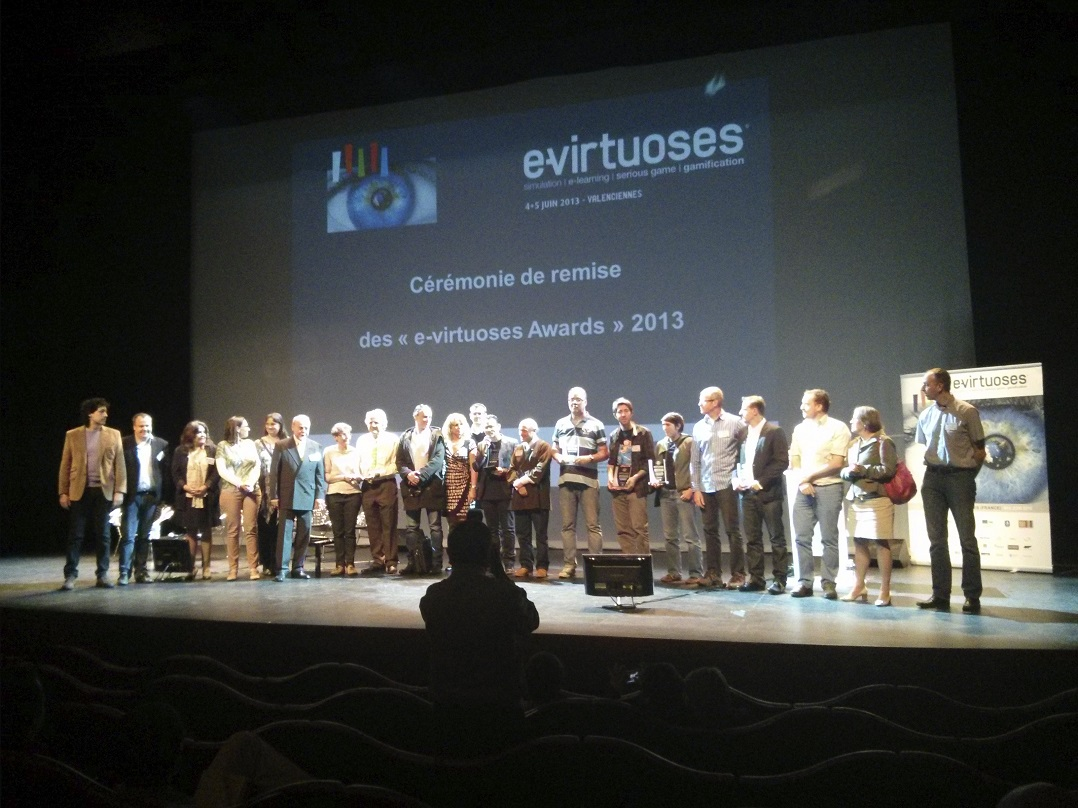
\includegraphics[width=210px, height=157px]{images/remise_awards_e-virtuoses_groupe.jpg}
			\caption{Gagnants des e-virtuoses 2013 dans les différentes catégories.}
			\label{Gagnants}
		\end{center}
	\end{minipage}
	\hfill
	\begin{minipage}[c]{.45\linewidth}
		\begin{center}
			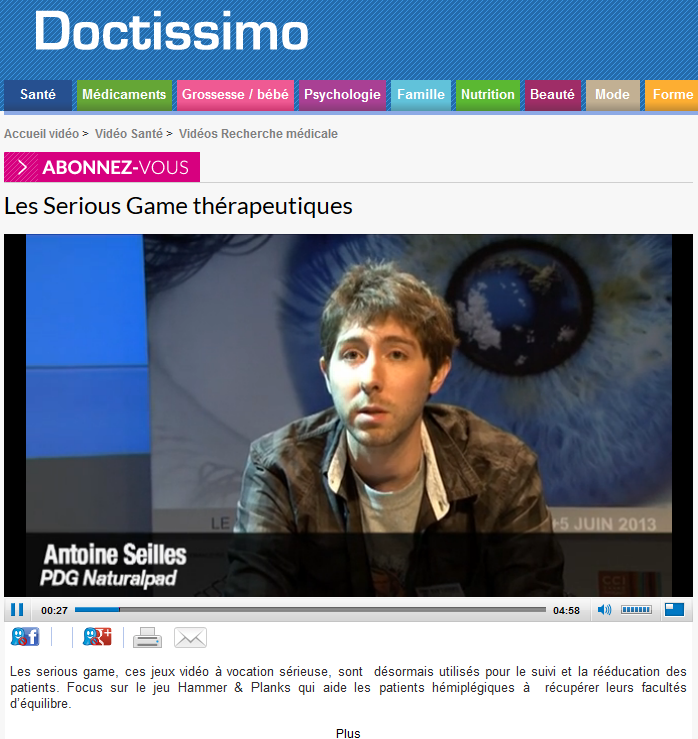
\includegraphics[height=157px]{images/doctissimo.png}
			\caption{Article de doctissimo sur les Serious game thérapeutiques.}
			\label{naturalpad_groupe}
		\end{center}
	\end{minipage}
\end{figure}		

Hammer \& Planks est constitué d’un environnement 3D vu de dessus. Le joueur contrôle un bateau qu'il peut déplacer de gauche à droite et de haut en bas, et peut éliminer les ennemis grâce à ses canons. Enfin, il doit éviter des obstacles et peut récupérer des bonus. Pour contrôler le bateau, il existe plusieurs solutions : on peut utiliser la Kinect, la Wii Board, une manette ou bien le clavier et la souris. Le jeu a initialement été conçu pour une utilisation avec la Wii Board afin de travailler les facultés d'équilibre, que ce soit assis ou debout. Le jeu possède par ailleurs un ensemble de paramètres qui peuvent être paramétrés ou changés en cours de partie, rendant ainsi le jeu devient ajustable selon les besoins thérapeutiques. On notera qu'il existe une version grand public du jeu, où la paramétrisation avancée est remplacée par un enrichissement du gameplay et du scénario notamment.
	\begin{figure}[!t]
		\centering
		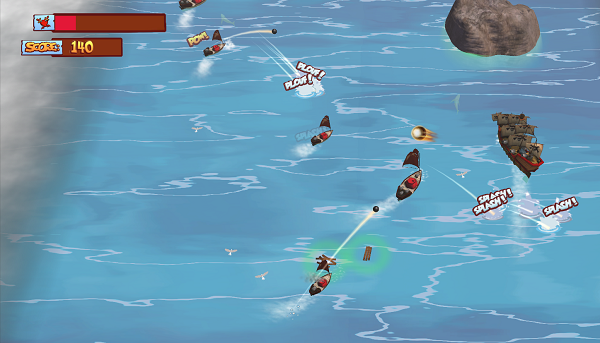
\includegraphics[width=420px]{images/hammer_and_planks.png}
		\caption{Impression d'écran du jeu Hammer \& Planks}
		A droite, le bateau contrôlé par le joueur.
		\label{hammer_and_planks}
	\end{figure}
